\documentclass{article}
% Change "article" to "report" to get rid of page number on title page
\usepackage{amsmath,amsfonts,amsthm,amssymb}
\usepackage{setspace}
\usepackage{Tabbing}
\usepackage{fancyhdr}
\usepackage{lastpage}
\usepackage{extramarks}
\usepackage{chngpage}
\usepackage{soul,color}
\usepackage{graphicx,float,wrapfig}
\usepackage{multirow}
\usepackage{enumerate}
% In case you need to adjust margins:
\topmargin=-0.45in      %
\evensidemargin=0in     %
\oddsidemargin=0in      %
\textwidth=6.5in        %
\textheight=9.0in       %
\headsep=0.25in         %

% Homework Specific Information
\newcommand{\hmwkTitle}{Finaally...Let there be bars}
\newcommand{\hmwkClass}{}
\newcommand{\hmwkAuthorName}{Donglai\ Wei}


% Setup the header and footer
\pagestyle{fancy}                                                       %
\lhead{\hmwkAuthorName}                                                 %
\rhead{\firstxmark}                                                     %
\lfoot{\lastxmark}                                                      %
\cfoot{}                                                                %
\rfoot{Page\ \thepage\ of\ \pageref{LastPage}}                          %
\renewcommand\headrulewidth{0.4pt}                                      %
\renewcommand\footrulewidth{0.4pt}                                      %

% This is used to trace down (pin point) problems
% in latexing a document:
%\tracingall

%%%%%%%%%%%%%%%%%%%%%%%%%%%%%%%%%%%%%%%%%%%%%%%%%%%%%%%%\begin{enumerate}

% Some tools
\newcommand{\enterProblemHeader}[1]{\nobreak\extramarks{#1}{#1 continued on next page\ldots}\nobreak%
                                    \nobreak\extramarks{#1 (continued)}{#1 continued on next page\ldots}\nobreak}%
\newcommand{\exitProblemHeader}[1]{\nobreak\extramarks{#1 (continued)}{#1 continued on next page\ldots}\nobreak%
                                   \nobreak\extramarks{#1}{}\nobreak}%

\newlength{\labelLength}
\newcommand{\labelAnswer}[2]
  {\settowidth{\labelLength}{#1}%
   \addtolength{\labelLength}{0.25in}%
   \changetext{}{-\labelLength}{}{}{}%
   \noindent\fbox{\begin{minipage}[c]{\columnwidth}#2\end{minipage}}%
   \marginpar{\fbox{#1}}%

   % We put the blank space above in order to make sure this
   % \marginpar gets correctly placed.
   \changetext{}{+\labelLength}{}{}{}}%

\setcounter{secnumdepth}{0}
\newcommand{\homeworkProblemName}{}%
\newcounter{homeworkProblemCounter}%
\newenvironment{homeworkProblem}[1][Problem \arabic{homeworkProblemCounter}]%
  {\stepcounter{homeworkProblemCounter}%
   \renewcommand{\homeworkProblemName}{#1}%
   \section{\homeworkProblemName}%
   \enterProblemHeader{\homeworkProblemName}}%
  {\exitProblemHeader{\homeworkProblemName}}%

\newcommand{\problemAnswer}[1]
  {\noindent\fbox{\begin{minipage}[c]{\columnwidth}#1\end{minipage}}}%

\newcommand{\problemLAnswer}[1]
  {\labelAnswer{\homeworkProblemName}{#1}}

\newcommand{\homeworkSectionName}{}%
\newlength{\homeworkSectionLabelLength}{}%
\newenvironment{homeworkSection}[1]%
  {% We put this space here to make sure we're not connected to the above.
   % Otherwise the changetext can do funny things to the other margin

   \renewcommand{\homeworkSectionName}{#1}%
   \settowidth{\homeworkSectionLabelLength}{\homeworkSectionName}%
   \addtolength{\homeworkSectionLabelLength}{0.25in}%
   \changetext{}{-\homeworkSectionLabelLength}{}{}{}%
   \subsection{\homeworkSectionName}%
   \enterProblemHeader{\homeworkProblemName\ [\homeworkSectionName]}}%
  {\enterProblemHeader{\homeworkProblemName}%

   % We put the blank space above in order to make sure this margin
   % change doesn't happen too soon (otherwise \sectionAnswer's can
   % get ugly about their \marginpar placement.
   \changetext{}{+\homeworkSectionLabelLength}{}{}{}}%

\newcommand{\sectionAnswer}[1]
  {% We put this space here to make sure we're disconnected from the previous
   % passage

   \noindent\fbox{\begin{minipage}[c]{\columnwidth}#1\end{minipage}}%
   \enterProblemHeader{\homeworkProblemName}\exitProblemHeader{\homeworkProblemName}%
   \marginpar{\fbox{\homeworkSectionName}}%

   % We put the blank space above in order to make sure this
   % \marginpar gets correctly placed.
   }%

%%%%%%%%%%%%%%%%%%%%%%%%%%%%%%%%%%%%%%%%%%%%%%%%%%%%%%%%%%%%%



%%%%%%%%%%%%%%%%%%%%%%%%%%%%%%%%%%%%%%%%%%%%%%%%%%%%%%%%%%%%%
% Make title
\title{\vspace{0.3in}\textmd{\textbf{\hmwkTitle}}}
\date{2010.5.28}
\author{\textbf{\hmwkAuthorName}}
%%%%%%%%%%%%%%%%%%%%%%%%%%%%%%%%%%%%%%%%%%%%%%%%%%%%%%%%%%%%%

\begin{document}
\begin{spacing}{1.1}
\maketitle

\section{0) Key Words}

\begin{enumerate}
\item  Light-version: of Split-Restaurant and Split-Dish for more runs
\item  Full-version: of Split-Dish and Split-Dish for robustness
\item  Split-Dish-All/Further: Bigger moves for Split-Dish
\item  Mixing Process: Better mixing Iterations between Split-Restaurant and Split-Dish for faster "convergence"
\item  Small Tricks: some little modifications for better split and merge moves.
\end{enumerate}


\section{1) Pseudocode}
For Initialization:\\
{\bf Table Config} is the key.\\
{\bf Aim}: Since dish config is vague, it is wise to just split Restaurant into smaller tables for later reconstruction.\\ \\
For Search:\\
{\bf Dish Config} is the key.\\
{\bf Aim}: Since table config is local,it is wise to focus on better Dish Config across restaurants.\\


\begin{enumerate}[(I)]
\item {\bf SCHEME}\\ \\
\begin{enumerate}[(a)]
 \item Initialization:\\
    1 table and 1 dish per restaurant\\
      Repeat several times:
       \begin{enumerate}[(1)]
        \item Run Split-Restaurant(Full-version)[accept]
	\item Run Split-Dish(Light-version)[accept](random Dish k)
      \end{enumerate}
\item Search:\\
  Repeat several times:
   \begin{enumerate}[(1)]
     \item Run Split-Restaurant(Light-Version)[accept/reject](random Restaurant j)
     \item Run Split-Dish(Full-Version)[accept/reject](random Dish k)
     \item (Occasionally)Run Split-Dish-All[accept/reject]
     \item (Occasionally)Run Split-Dish-Further[accept/reject](random Dish k)
    \end{enumerate}

\end{enumerate}
\item {\bf Split-Restaurant}
\begin{enumerate}[(a)]
 \item Light-Version[Decision](j)
\begin{enumerate}[(1)]
\item In random order,Split all tables in j using 2-means++(producing 2$m_{j.}$ initial tables)
\item Run TKM search(Local Search table/dish+Merge table)
\item Decision for the new config
\end{enumerate}
 \item Full-Version[Decision]
\begin{enumerate}[(1)]
\item For j=randperm(J)
\item In random order,Split all tables in j using 2-means++(producing 2$m_{j.}$ initial tables)
\item Run TKM search(Local Search table/dish)
\item Decision for the new config
\item End
\end{enumerate}

\end{enumerate}
\item {\bf Split-Dish}
\begin{enumerate}[(a)]
 \item Light-Version[Decision](k)
\begin{enumerate}[(1)]
\item In random order,Split all tables in dish k using 2-means++(producing 2$m_{.k}$ initial tables) 
\item Split dish k using 2-means++
\item Run TKM search(Local Search table/dish)
\item Decision for the new config
\end{enumerate}
 \item Full-Version[Decision](k)
\begin{enumerate}[(1)]
\item In random order,Split all tables in dish k using 2-means++(producing 2$m_{.k}$ initial tables) 
\item (Multiple Runs)Split dish k using 2-means++
\item (Multiple Runs)Run TKM search(Local Search table/dish+merge dish)(?merge table)
\item Decision for the new config
\end{enumerate}
\item All-Version[Decision]
\begin{enumerate}[(1)]
\item For k=randperm(K)
\item if(k$leq$length(dishes))
\item Light-Version Split-Dishes[accept](k)
\item End
\item End
\item (Multiple Runs)Run TKM search(Local Search table/dish+merge dish)
\item Decision for the new configuration
\end{enumerate}
\item Further-Version[Decision](k)
\begin{enumerate}[(1)]
\item Full-Version Split-Dishes[accept](k)\\
 d1,d2 are the dishes that the splitted dishes are assigned to
\item If(d1$\neq$d2)
\item Further-Version Split-Dishes[accept](d1)
\item Further-Version Split-Dishes[accept](d2)
\item End
\item (Multiple Runs)Run TKM search(Local Search table/dish+merge dish)
\item Decision for the new configuration
\end{enumerate}

\end{enumerate}
\item {\bf TKM}
While log probability does not increase any more:
\begin{enumerate}[(1)]
\item Local Search Tables(For chosen restaurants)
\item Local Search Dishes(For chosen dishes)
\item Merge Tables(For chosen restaurants)
\item Merge Dishes(For chosen dishes)
\end{enumerate}

\item {\bf Small Tricks}
\begin{enumerate}[(1)]
\item Merge Dish:
\begin{enumerate}[(i)]
\item Previously: Simply Merge two dishes without changing table config
\item Better:Given Dish config$\vec k_{jt}$(k-term fixed), it is better to merge tables(belong to dish k) in the same restaurant to further decrease -log Probability.
\end{enumerate}
\item Split table:
\begin{enumerate}[(i)]
\item Previously: 2-means++ allows new tables to have new/previous dishes
\item Better:During Search, in order to split "sticky" table/dish, it is better not to allow them assigned to new/previous dishes.
\end{enumerate}
\item Split dish:(similar to Split table) 
\end{enumerate}
\end{enumerate}



\section{2) Experiment}
\subsection{i)Settings}
40 Restaurants,10 bars\\ \\ \\ \\ \\ \\ \\ \\ \\ \\ \\
\begin{figure}
    \centering 
    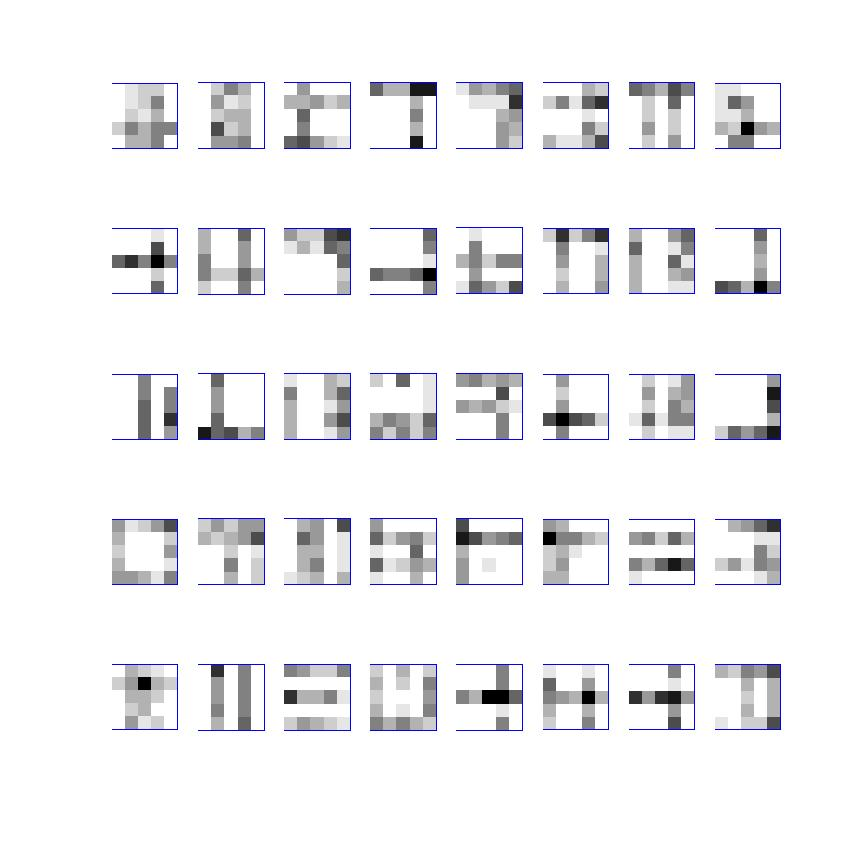
\includegraphics[width=1.5in,height=1.5in]{restau.jpg} 
    \caption{40 Restaurants}
\end{figure}

\subsection{ii) Initialization}
Run 5 times:Split-Restaurant(Full-Version) + Split-Dish(Light-Version)
\begin{figure}[h] 
  \begin{minipage}[b]{0.5\textwidth} 
    \centering 
    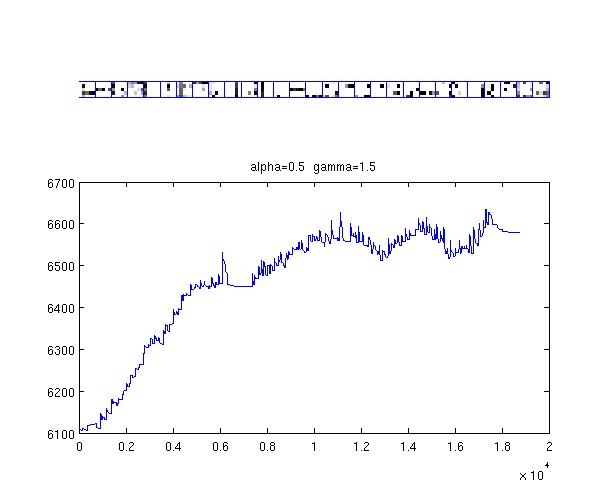
\includegraphics[width=2.5in,height=2in]{init1_5.jpg} 
    \caption{5 runs:Dish Config and -log Probability}
    \label{fig:by:table} 
  \end{minipage}% 
  \begin{minipage}[b]{0.5\textwidth} 
    \centering 
    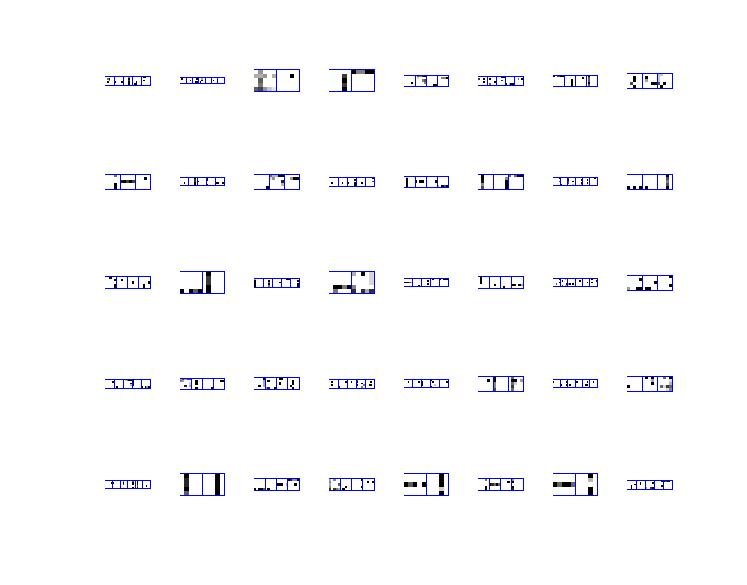
\includegraphics[width=2.5in,height=2in]{init1_5d.jpg} 
    \caption{5 runs:Table Config for 40 restaurants}
    \label{fig:by:table}  
   \end{minipage}% 
\end{figure}

\subsection{iii) Search}

{\bf Outline:}
\begin{enumerate}
\item {\bf Scheme 1:Split-Restaurant:Split-Dish=1:1}
\item {\bf Scheme 2:Split-Restaurant:Split-Dish=5:1}
\item {\bf Bigger Moves:Split-Dish(All-Version)+(Further-Version)}
\end{enumerate}
1) For j=randperm(J) 
\begin{enumerate}
\item Split-Restaurant(Light-Version) 
\item Split-Dish(Full-Version)
\end{enumerate}
End\\ \\
Two variants:\\
a)Split-Dish(Full-Version) with merge tables in TKM\\
b)Split-Dish(Full-Version) with merge tables in TKM\\ \\
{\bf Conclusion:}\\I tried several runs and found a) in the beginning tends to create single table for the restaurant since the 
dish config is still vague(t-term dominates).\\
Below are the typical examples.
\begin{figure}[h] 
  \begin{minipage}[b]{0.5\textwidth} 
    \centering 
    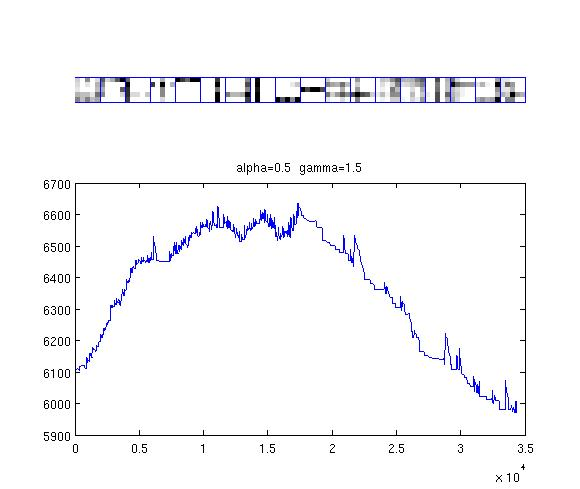
\includegraphics[width=2.5in,height=2in]{init1_5_mt40.jpg} 
    \caption{a) with merge table:Dish Config and -log Probability}
    \label{fig:by:table} 
  \end{minipage}% 
  \begin{minipage}[b]{0.5\textwidth} 
    \centering 
    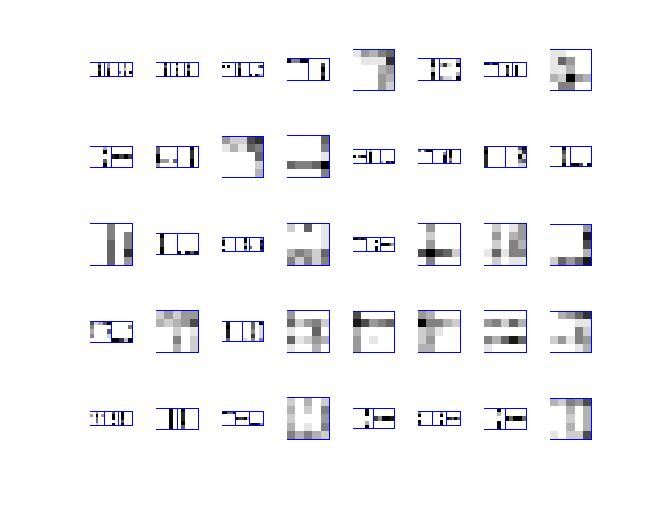
\includegraphics[width=2.5in,height=2in]{init1_5_mt40d.jpg} 
    \caption{a) with merge table:Table Config for 40 restaurants}
    \label{fig:by:table}  
   \end{minipage}% 
\end{figure}
\begin{figure}[h] 
  \begin{minipage}[b]{0.5\textwidth} 
    \centering 
    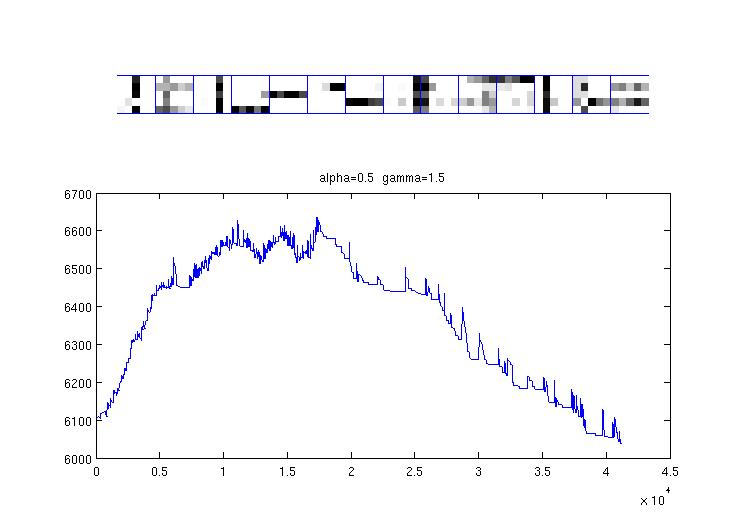
\includegraphics[width=2.5in,height=2in]{init1_5_nmt40.jpg} 
    \caption{b) without merge table:Dish Config and -log Probability}
    \label{fig:by:table} 
  \end{minipage}% 
  \begin{minipage}[b]{0.5\textwidth} 
    \centering 
    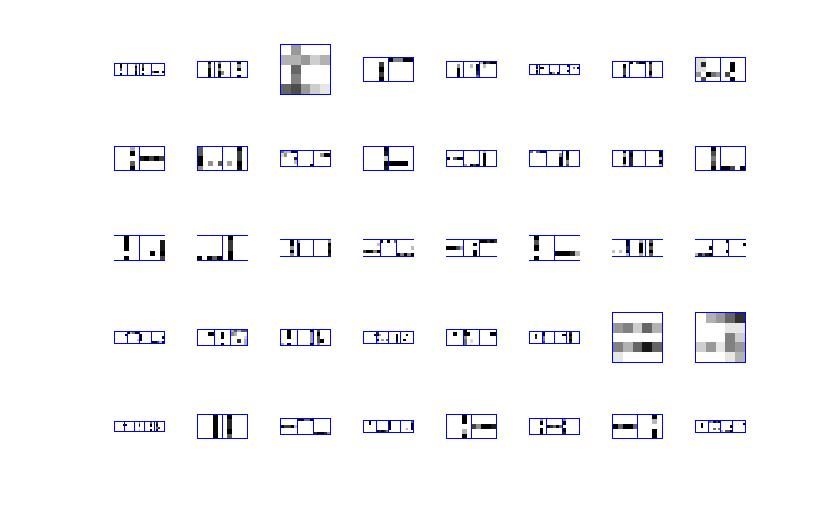
\includegraphics[width=2.5in,height=2in]{init1_5_nmt40d.jpg} 
    \caption{b) without merge table:Table Config for 40 restaurants}
    \label{fig:by:table}  
   \end{minipage}% 
\end{figure}
\\ \\ \\ \\ \\ \\ \\ \\ \\ \\ \\ \\ \\ 
2)Since Split-Dish(Full-Version) is expensive and may not benefit much from one Split-Restaurant(Light-Version), we may try the mixing process below:
(No merge table during TKM in Split-Dish(Full-Version))\\ \\
For Iter=1:5\\
count=1;\\
For j=randperm(J) 
\begin{enumerate}
\item Split-Restaurant(Light-Version) 
\item If(mode(count,5)==0)\\
Split-Dish(Full-Version)\\
End
\item count=count+1;
\end{enumerate}
End\\
End\\
\begin{figure}[h] 
  \begin{minipage}[b]{0.5\textwidth} 
    \centering 
    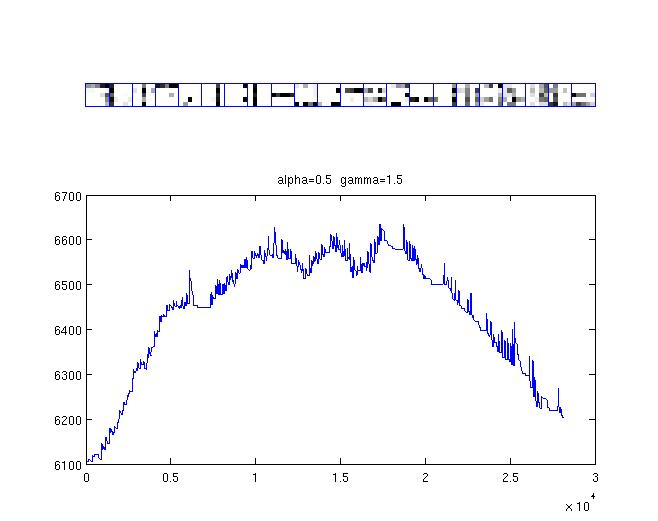
\includegraphics[width=2.5in,height=2in]{init1_5_nmt85.jpg} 
    \caption{Iter 1:Dish Config and -log Probability}
    \label{fig:by:table} 
  \end{minipage}% 
  \begin{minipage}[b]{0.5\textwidth} 
    \centering 
    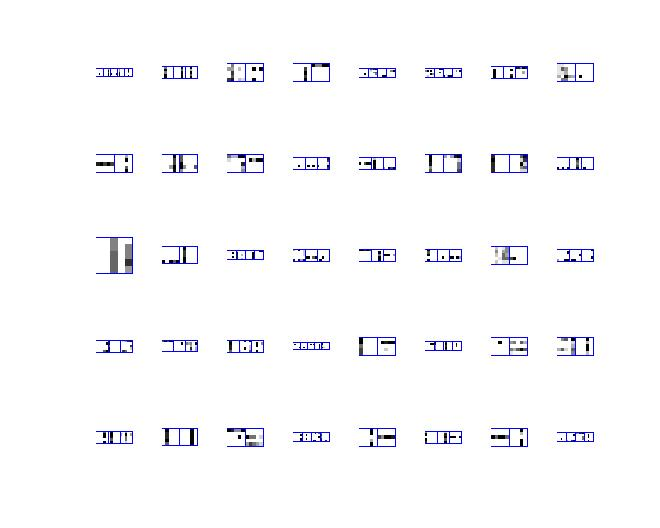
\includegraphics[width=2.5in,height=2in]{init1_5_nmt85d.jpg} 
    \caption{Iter 1:Table Config for 40 restaurants}
    \label{fig:by:table}  
   \end{minipage}% 
\end{figure}
\begin{figure}[h] 
  \begin{minipage}[b]{0.5\textwidth} 
    \centering 
    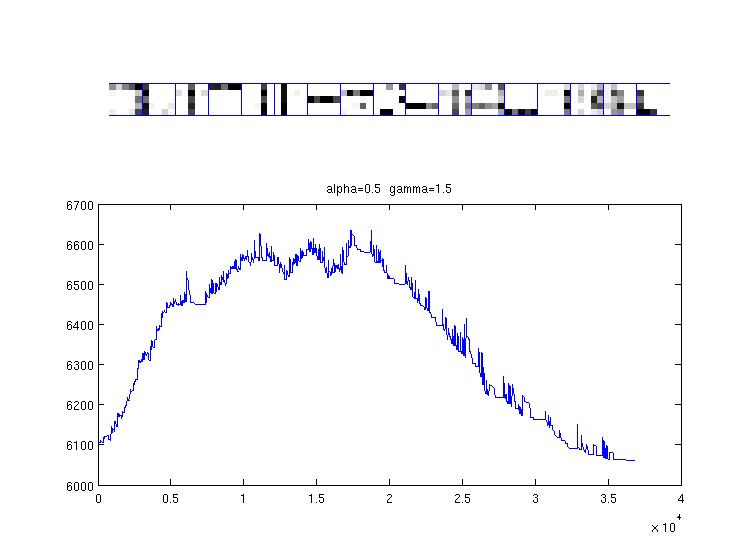
\includegraphics[width=2.5in,height=2in]{init1_5_nmt85_2d.jpg} 
    \caption{Iter 2:Dish Config and -log Probability}
    \label{fig:by:table} 
  \end{minipage}% 
  \begin{minipage}[b]{0.5\textwidth} 
    \centering 
    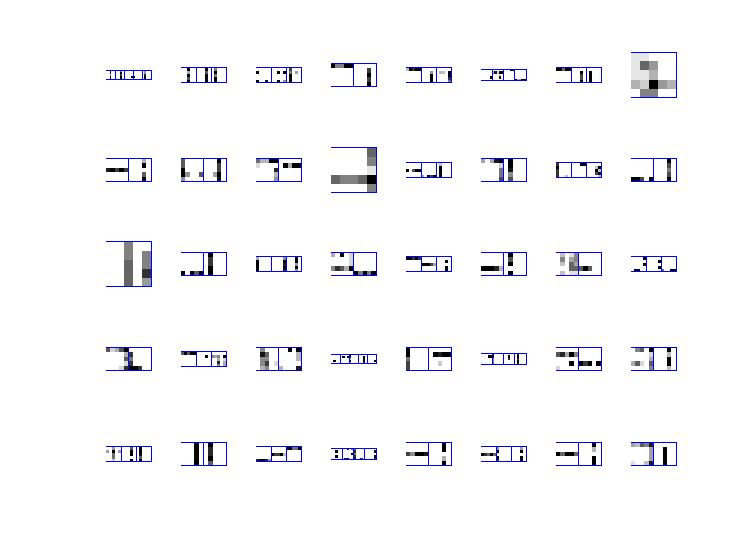
\includegraphics[width=2.5in,height=2in]{init1_5_nmt85_2.jpg} 
    \caption{Iter 2:Table Config for 40 restaurants}
    \label{fig:by:table}  
   \end{minipage}% 
\end{figure}
\begin{figure}[h] 
  \begin{minipage}[b]{0.5\textwidth} 
    \centering 
    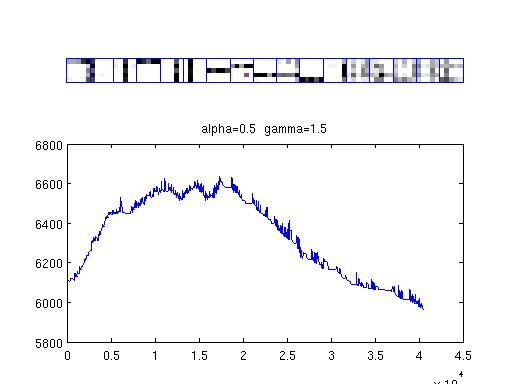
\includegraphics[width=2.5in,height=2in]{init1_5_nmt85_3d.jpg} 
    \caption{Iter 3:Dish Config and -log Probability}
    \label{fig:by:table} 
  \end{minipage}% 
  \begin{minipage}[b]{0.5\textwidth} 
    \centering 
    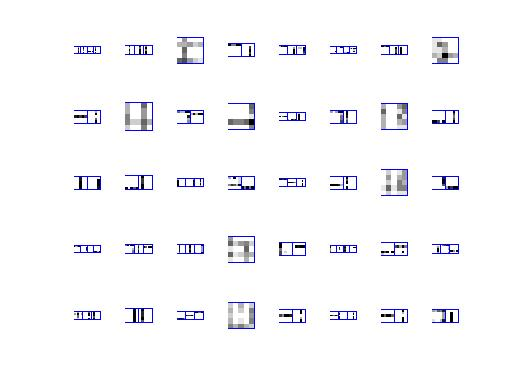
\includegraphics[width=2.5in,height=2in]{init1_5_nmt85_3.jpg} 
    \caption{Iter 3:Table Config for 40 restaurants}
    \label{fig:by:table}  
   \end{minipage}% 
\end{figure}
\begin{figure}[h] 
  \begin{minipage}[b]{0.5\textwidth} 
    \centering 
    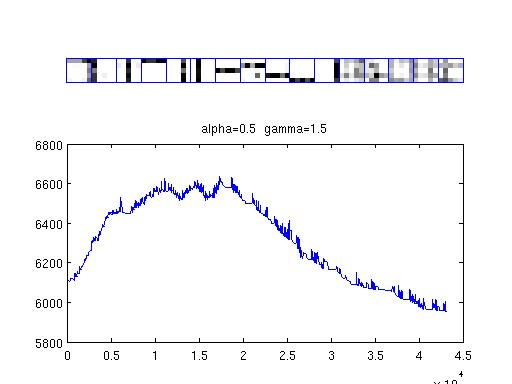
\includegraphics[width=2.5in,height=2in]{init1_5_nmt85_4d.jpg} 
    \caption{Iter 4:Dish Config and -log Probability}
    \label{fig:by:table} 
  \end{minipage}% 
  \begin{minipage}[b]{0.5\textwidth} 
    \centering 
    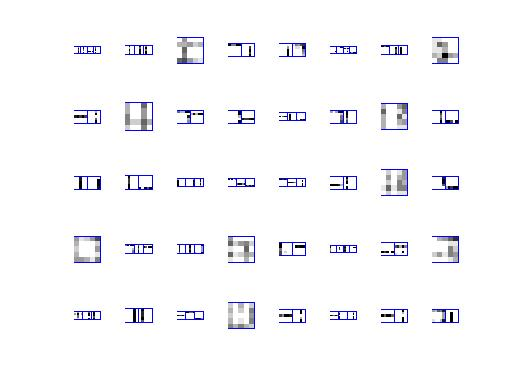
\includegraphics[width=2.5in,height=2in]{init1_5_nmt85_4.jpg} 
    \caption{Iter 4:Table Config for 40 restaurants}
    \label{fig:by:table}  
   \end{minipage}% 
\end{figure}
\begin{figure}[h] 
  \begin{minipage}[b]{0.5\textwidth} 
    \centering 
    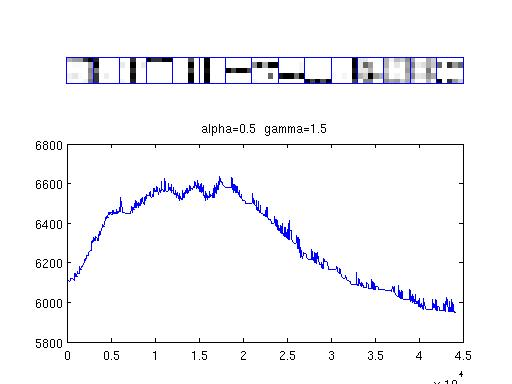
\includegraphics[width=2.5in,height=2in]{init1_5_nmt85_5d.jpg} 
    \caption{Iter 5:Dish Config and -log Probability}
    \label{fig:by:table} 
  \end{minipage}% 
  \begin{minipage}[b]{0.5\textwidth} 
    \centering 
    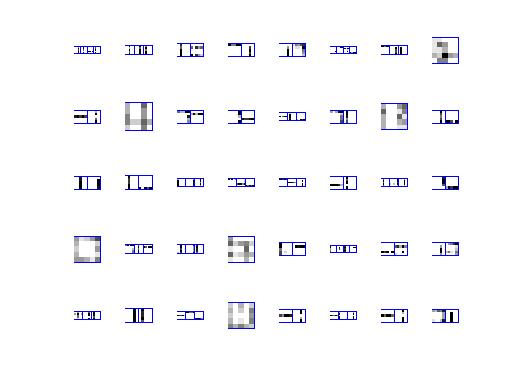
\includegraphics[width=2.5in,height=2in]{init1_5_nmt85_5.jpg} 
    \caption{Iter 5:Table Config for 40 restaurants}
    \label{fig:by:table}  
   \end{minipage}% 
\end{figure}
\\ \\ \\ \\ \\ \\ \\ \\ \\ \\ \\ \\ \\ \\ \\ \\ \\ \\ \\ \\ \\ \\ \\ \\ \\ \\ \\ \\ \\ \\ \\ \\ \\ \\ \\ \\ \\ \\ \\ \\ \\ \\ \\ \\ \\ \\ \\ \\ \\ \\ \\ \\ \\ \\ \\ \\
3)From Above, though we roughly figure out 10 true bars, the noisy dishes refuse to be "explained" by them.\\
The reason is manyfold:\\
\begin{enumerate}
\item Some of the true bars are not "strong enough":though splitting one noisy dish decreases k-term, the t-term increases more.  
\item The noisy dish is composed of more than two bars, thus split it into two components may not be better than leave it alone.
\end{enumerate}
Possible Solutions:\\
\begin{enumerate}
\item Split-Dish-All: though split one noisy dish may be weak, we can wait and accumulate them. In the end, it may be profitable.
\item Split-Dish-Further:Split-Dish(Full version)(k)+Split-Dish(Further version)(d1,d2)\\
(p.s. we expect true bars won't be bothered by it:true bars may not be well explained by two other dishes, thus 2-means++ will assign )
\end{enumerate}
Thus, we have following Scheme:\\ \\
While -log probability cannot decrease any more\\
count=1;\\
For j=randperm(J) 
\begin{enumerate}
\item Split-Restaurant(Light-Version)[accept/reject](j)
\item If(mode(count,5)==0)\\
Split-Dish(Full-Version)[accept/reject]\\
End
\item count=count+1;
\end{enumerate}
End\\
Split-Dish(All-Version)[accept/reject]\\
Split-Dish(Further-Version)[accept/reject](random k)\\
End\\

\begin{figure}[h] 
  \begin{minipage}[b]{0.5\textwidth} 
    \centering 
    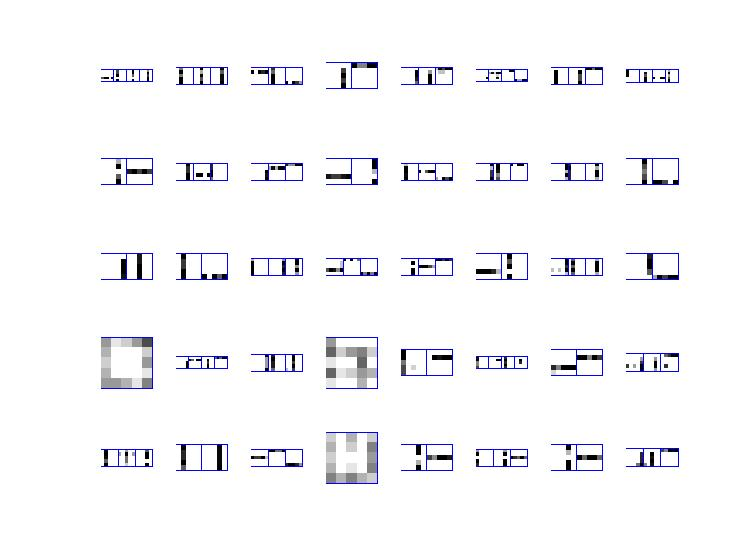
\includegraphics[width=2.5in,height=2in]{init1_5_nmt85_allll.jpg} 
    \caption{Iterations with Split-Dish(All-Version) only}
    \label{fig:by:table} 
  \end{minipage}% 
  \begin{minipage}[b]{0.5\textwidth} 
    \centering 
    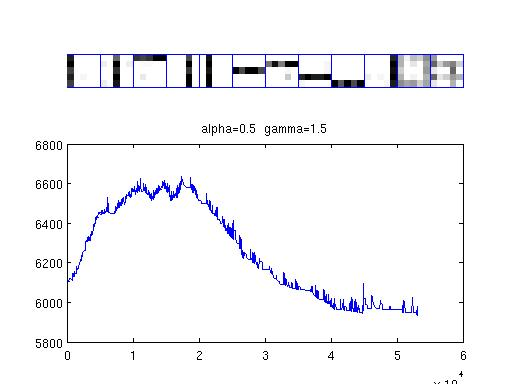
\includegraphics[width=2.5in,height=2in]{init1_5_nmt85_allll_d.jpg} 
    \caption{dish config for Fig 18:The last 2 dishes are problematic}
    \label{fig:by:table}  
   \end{minipage}% 
\end{figure}

\begin{figure}[h] 
  \begin{minipage}[b]{0.5\textwidth} 
    \centering 
    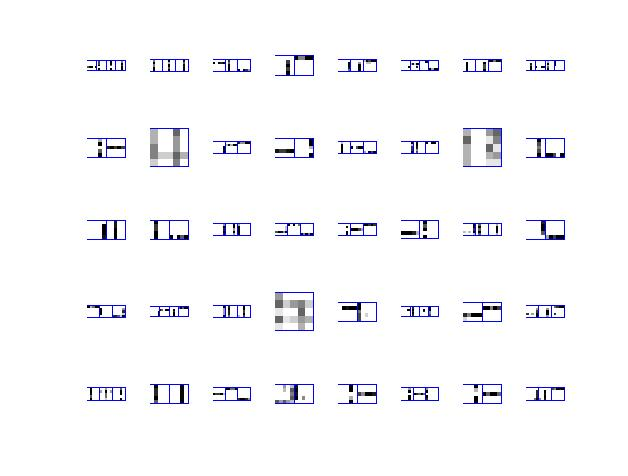
\includegraphics[width=2.5in,height=2in]{init1_5_nmt85_fur1.jpg} 
    \caption{+Split-Dish(Further-Version):Get out of stuck while introducing new noise}
    \label{fig:by:table} 
  \end{minipage}% 
    \begin{minipage}[b]{0.5\textwidth} 
    \centering 
    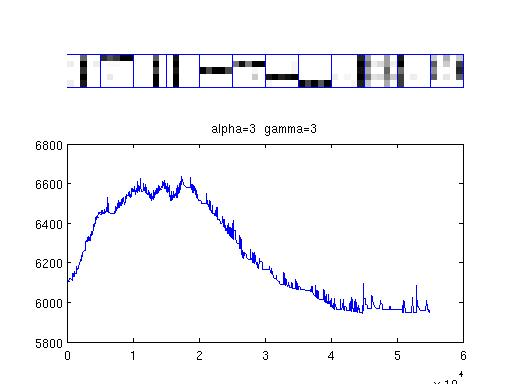
\includegraphics[width=2.5in,height=2in]{init1_5_nmt85_fur3.jpg} 
    \caption{dish config for Fig 20:alleviate the problem by introducing new dishes}
    \label{fig:by:table} 
  \end{minipage}% 
\end{figure}
\begin{figure}[h] 
  \begin{minipage}[b]{0.5\textwidth} 
    \centering 
    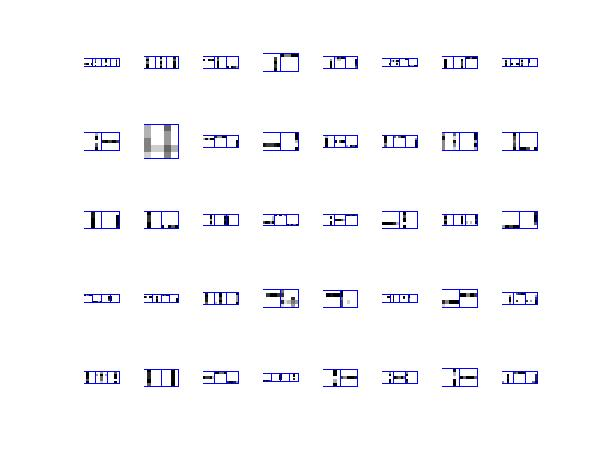
\includegraphics[width=2.5in,height=2in]{init1_5_nmt85_fur4_re.jpg} 
    \caption{+Split-Dish(Further-Version): get rid of the last dish}
    \label{fig:by:table} 
  \end{minipage}% 
  \begin{minipage}[b]{0.5\textwidth} 
    \centering 
    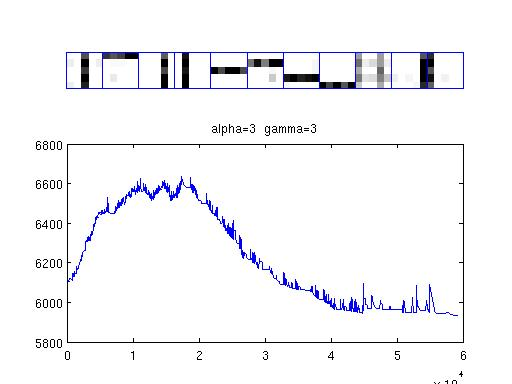
\includegraphics[width=2.5in,height=2in]{init1_5_nmt85_fur4.jpg} 
    \caption{dish config for Fig 20:ALMOST THERE}
    \label{fig:by:table}  
   \end{minipage}% 
\end{figure}
\begin{figure}[h] 
  \begin{minipage}[b]{0.5\textwidth} 
    \centering 
    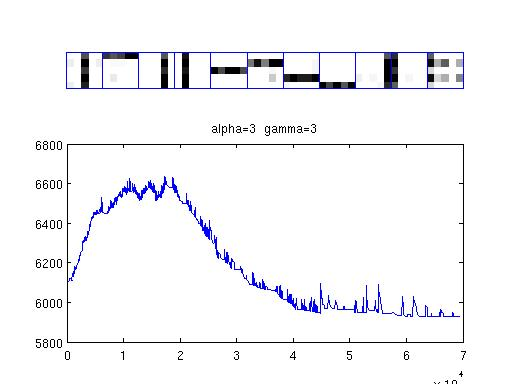
\includegraphics[width=2.5in,height=2in]{init1_5_nmt85_fur4_re_all.jpg} 
    \caption{+Split-Dish(All-Version): One more try}
    \label{fig:by:table} 
  \end{minipage}% 
  \begin{minipage}[b]{0.5\textwidth} 
    \centering 
    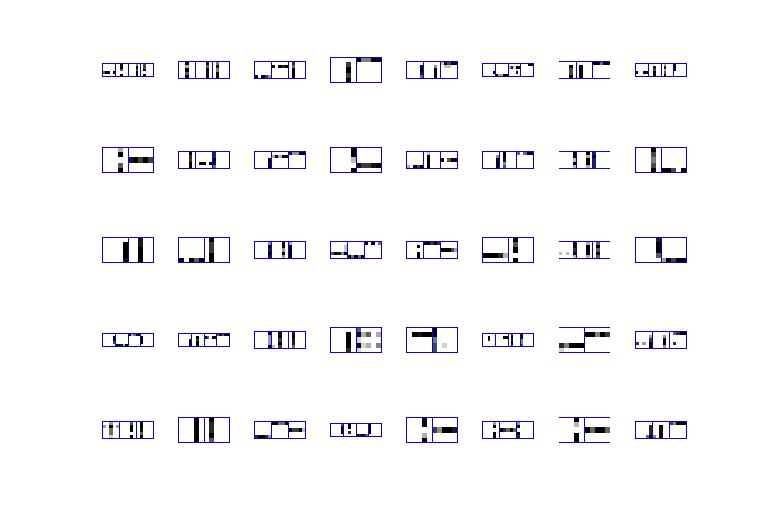
\includegraphics[width=2.5in,height=2in]{init1_5_nmt85_fur4_re_alld.jpg} 
    \caption{dish config for Fig 22:Closer}
    \label{fig:by:table}  
   \end{minipage}% 
\end{figure}

\begin{figure}[h] 
  \begin{minipage}[b]{0.5\textwidth} 
    \centering 
    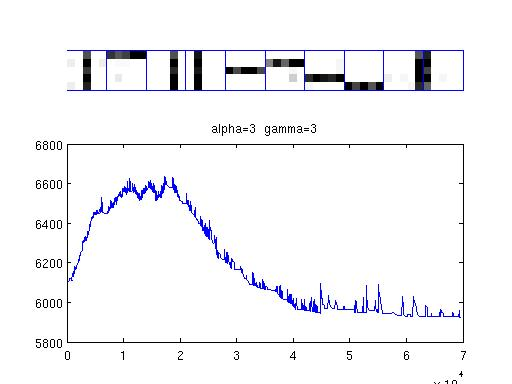
\includegraphics[width=2.5in,height=2in]{finald.jpg} 
    \caption{+Split-Restaurant}
    \label{fig:by:table} 
  \end{minipage}% 
  \begin{minipage}[b]{0.5\textwidth} 
    \centering 
    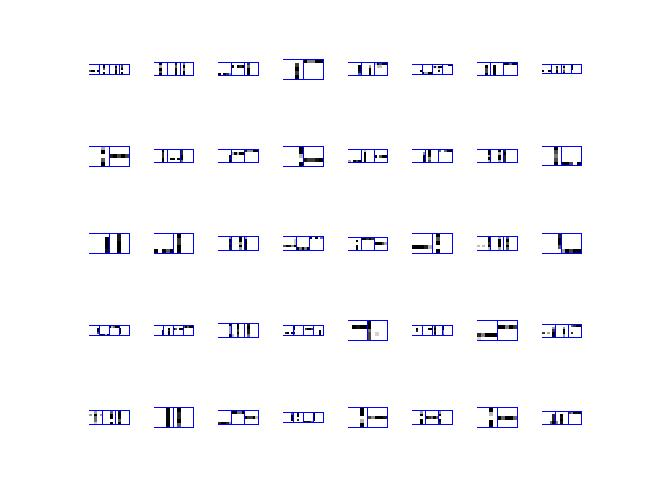
\includegraphics[width=2.5in,height=2in]{final.jpg} 
    \caption{dish config for Fig 24:Finally...}
    \label{fig:by:table}  
   \end{minipage}% 
\end{figure}


\end{spacing}
\end{document}

%%%%%%%%%%%%%%%%%%%%%%%%%%%%%%%%%%%%%%%%%%%%%%%%%%%%%%%%%%%%%
